%%%%%%%%%%%%%%%%%%%%%%%%%%%%%%%%%%%%%%%%%%%%%%%%%%%%%%%%%%%%%%%%%%%%%%%%%%%%%%%
% File: chopper_calibration_guide_ornl.tex
% Authors: EQSANS Instrument Team
% Date: March 2026
%
% ORNL TM format guide for EQSANS chopper calibration tools
%%%%%%%%%%%%%%%%%%%%%%%%%%%%%%%%%%%%%%%%%%%%%%%%%%%%%%%%%%%%%%%%%%%%%%%%%%%%%%%
\documentclass[tm]{ornltm}

%% Required packages
\usepackage{booktabs}
\usepackage{listings}
\usepackage{xcolor}

%% Define code listing style
\lstset{
    basicstyle=\ttfamily\small,
    backgroundcolor=\color{gray!10},
    frame=single,
    breaklines=true,
    columns=fullflexible,
    keepspaces=true
}

%%%%%%%%%%%%%%%%%%%%%%%%%%%%%%%%%%%%%%%%%%%%%%%%%%%%%%%%%%%%%%%%%%%%%%%%%%%%%%%
% AUTHORSHIP & PUBLISHING
%%%%%%%%%%%%%%%%%%%%%%%%%%%%%%%%%%%%%%%%%%%%%%%%%%%%%%%%%%%%%%%%%%%%%%%%%%%%%%%

\author{Changwoo Do \and Gergely Nagy \and William Heller \and Carrie Gao}

\title{EQSANS Chopper Calibration Tools\\[0.5em]
User Guide and Phase Offset Determination}

\reportnum{ORNL/TM-2026/XXX}
\division{Neutron Scattering Division}
\date{\today}

\reportdraft

%%%%%%%%%%%%%%%%%%%%%%%%%%%%%%%%%%%%%%%%%%%%%%%%%%%%%%%%%%%%%%%%%%%%%%%%%%%%%%%
% ABBREVIATIONS
%%%%%%%%%%%%%%%%%%%%%%%%%%%%%%%%%%%%%%%%%%%%%%%%%%%%%%%%%%%%%%%%%%%%%%%%%%%%%%%
\input{abbreviations.tex}

%%%%%%%%%%%%%%%%%%%%%%%%%%%%%%%%%%%%%%%%%%%%%%%%%%%%%%%%%%%%%%%%%%%%%%%%%%%%%%%
% DOCUMENT BODY
%%%%%%%%%%%%%%%%%%%%%%%%%%%%%%%%%%%%%%%%%%%%%%%%%%%%%%%%%%%%%%%%%%%%%%%%%%%%%%%
\begin{document}
\frontmatter

\tableofcontents
\listoffigures
\listoftables
\printacronyms

\mainmatter
\begin{abstract}
This guide describes the Python-based tools for \ac{eqsans} chopper calibration and phase verification at the \ac{sns}. The two primary tools are \texttt{find\_edges\_ui.py} for extracting phase offsets from experimental monitor spectra, and \texttt{eqsans\_chopper\_sim.py} for simulating multi-chopper neutron transmission and verifying phase configurations. This document provides step-by-step workflows, explains the underlying physics, and includes practical examples for both 60\,Hz and 30\,Hz operating modes.
\end{abstract}

\acresetall

%%%%%%%%%%%%%%%%%%%%%%%%%%%%%%%%%%%%%%%%%%%%%%%%%%%%%%%%%%%%%%%%%%%%%%%%%%%%%%%
\section{INTRODUCTION}
%%%%%%%%%%%%%%%%%%%%%%%%%%%%%%%%%%%%%%%%%%%%%%%%%%%%%%%%%%%%%%%%%%%%%%%%%%%%%%%

The \ac{eqsans} instrument at \ac{sns} uses a system of six disk choppers (1a, 1b, 2a, 2b, 3a, 3b) to define the wavelength band transmitted to the sample and detector. Precise timing (phase) of each chopper is critical for:
\begin{itemize}
    \item Selecting the desired wavelength range
    \item Minimizing frame overlap from adjacent source pulses
    \item Enabling frame-skip mode for extended wavelength coverage at 30\,Hz
\end{itemize}

The calibration workflow involves two complementary approaches:
\begin{enumerate}
    \item \textbf{Experimental measurement}: Using \texttt{find\_edges\_ui.py} to analyze monitor spectra and extract the actual chopper phase offsets from measured TOF edges.
    \item \textbf{Simulation verification}: Using \texttt{eqsans\_chopper\_sim.py} to predict the wavelength bands for given phase settings and verify consistency with the control system (hexaSub).
\end{enumerate}

%%%%%%%%%%%%%%%%%%%%%%%%%%%%%%%%%%%%%%%%%%%%%%%%%%%%%%%%%%%%%%%%%%%%%%%%%%%%%%%
\section{PHYSICAL BACKGROUND}
%%%%%%%%%%%%%%%%%%%%%%%%%%%%%%%%%%%%%%%%%%%%%%%%%%%%%%%%%%%%%%%%%%%%%%%%%%%%%%%

\subsection{Chopper Timing and TOF}

Neutrons travel from the moderator to each chopper with time-of-flight (TOF) determined by their wavelength $\lambda$ and the chopper distance $L$:
\begin{equation}
    \text{TOF} = \frac{L \cdot \lambda}{h/m_n} = \frac{L \cdot \lambda}{3956\,\text{m\,\AA/ms}}
\end{equation}

Each chopper has an opening gap characterized by:
\begin{itemize}
    \item \textbf{Opening angle} $\theta$: The angular width of the gap (in degrees)
    \item \textbf{OGC (Opening Gap Center)}: The time when the center of the gap aligns with the beam
    \item \textbf{Opening time}: $t_{\text{open}} = (\theta/360°) \times T_{\text{period}}$
\end{itemize}

\subsection{Chopper Configuration}

Table~\ref{tab:choppers} lists the \ac{eqsans} chopper parameters.

\begin{table}[ht]
\centering

\caption{\ac{eqsans} Chopper Parameters}
\label{tab:choppers}
\begin{tabular}{lccc}
\toprule
Chopper & Distance (m) & Opening (°) & Opening at 60\,Hz ($\mu$s) \\
\midrule
1a & 5.6601 & 129.605 & 6000 \\
1b & 5.6758 & 129.605 & 6000 \\
2a & 7.7601 & 179.989 & 8333 \\
2b & 7.7758 & 179.989 & 8333 \\
3a & 9.4978 & 230.010 & 10648 \\
3b & 9.5078 & 230.007 & 10648 \\
\bottomrule
\end{tabular}

\end{table}

\subsection{60\,Hz vs 30\,Hz Operation}

\textbf{60\,Hz mode}: Choppers rotate at 60\,Hz (period = 16,667\,$\mu$s), synchronized with the \ac{sns} source frequency. Each chopper opening window accepts neutrons from a single source pulse. Figure~\ref{fig:diagram_60hz} shows a distance--time diagram for 60\,Hz operation with a 2.5\,\AA{} starting wavelength.

\begin{figure}[ht]
    \centering
    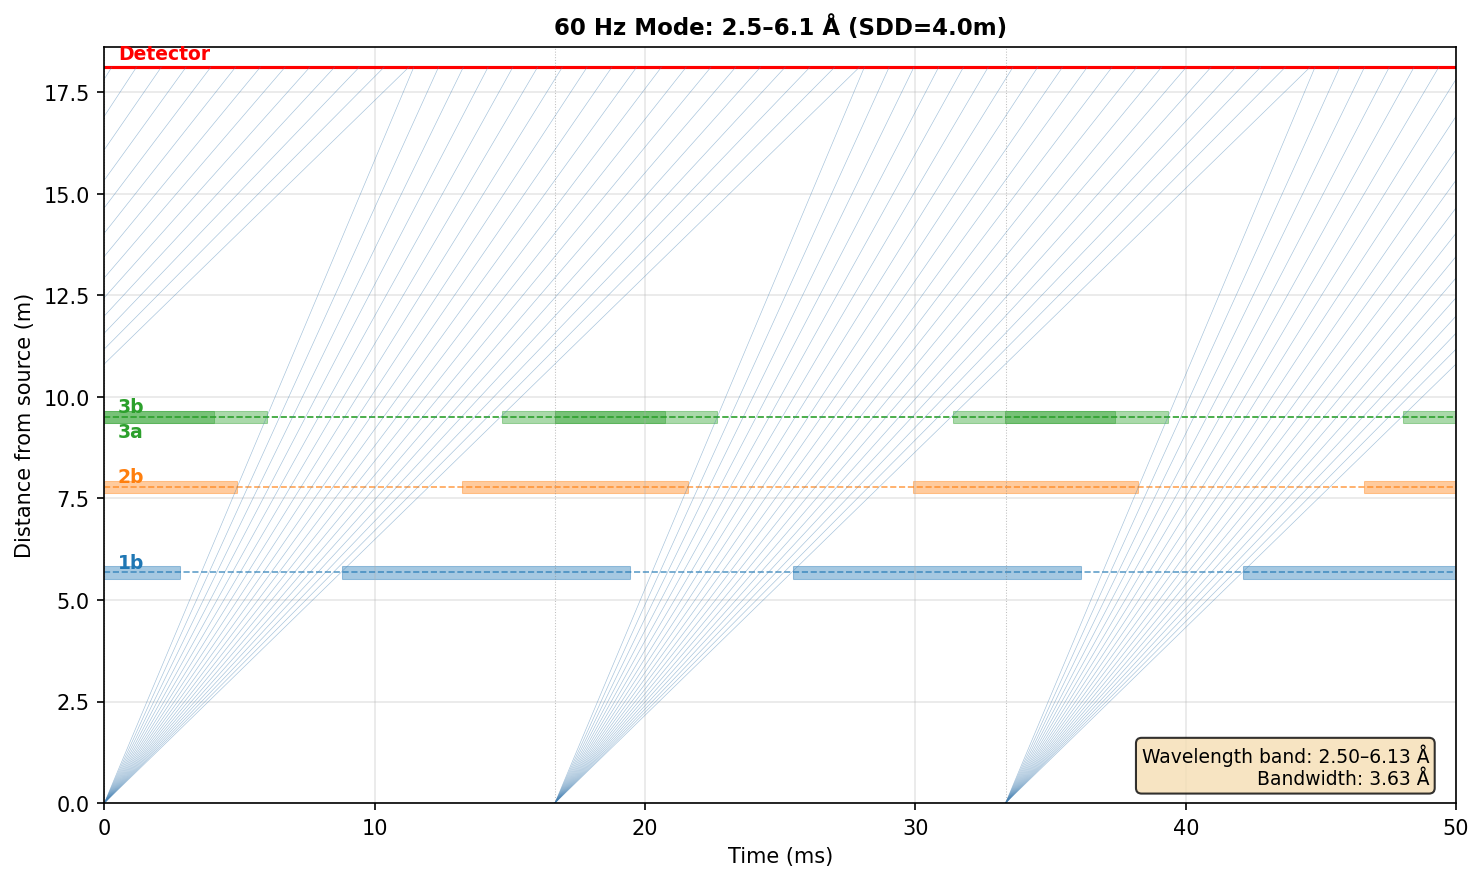
\includegraphics[width=5.5in]{figures/diagram_60hz.png}
    \longcaption{Distance--time diagram for 60\,Hz mode (2.5--6.1\,\AA{} band).}{Shaded rectangles indicate chopper closed periods. Blue trajectories show neutrons that successfully pass through all four choppers (1b, 2b, 3a, 3b).}
    \label{fig:diagram_60hz}
\end{figure}

\textbf{30\,Hz mode (frame-skip)}: Choppers rotate at 30\,Hz (period = 33,333\,$\mu$s), but the source still operates at 60\,Hz. This creates two wavelength bands per chopper cycle:
\begin{itemize}
    \item \textbf{Band 1}: Neutrons from the ``current'' source pulse
    \item \textbf{Band 2}: Neutrons from the ``previous'' source pulse (16.67\,ms earlier)
\end{itemize}

Figure~\ref{fig:diagram_30hz} illustrates the frame-skip configuration.

\begin{figure}[ht]
    \centering
    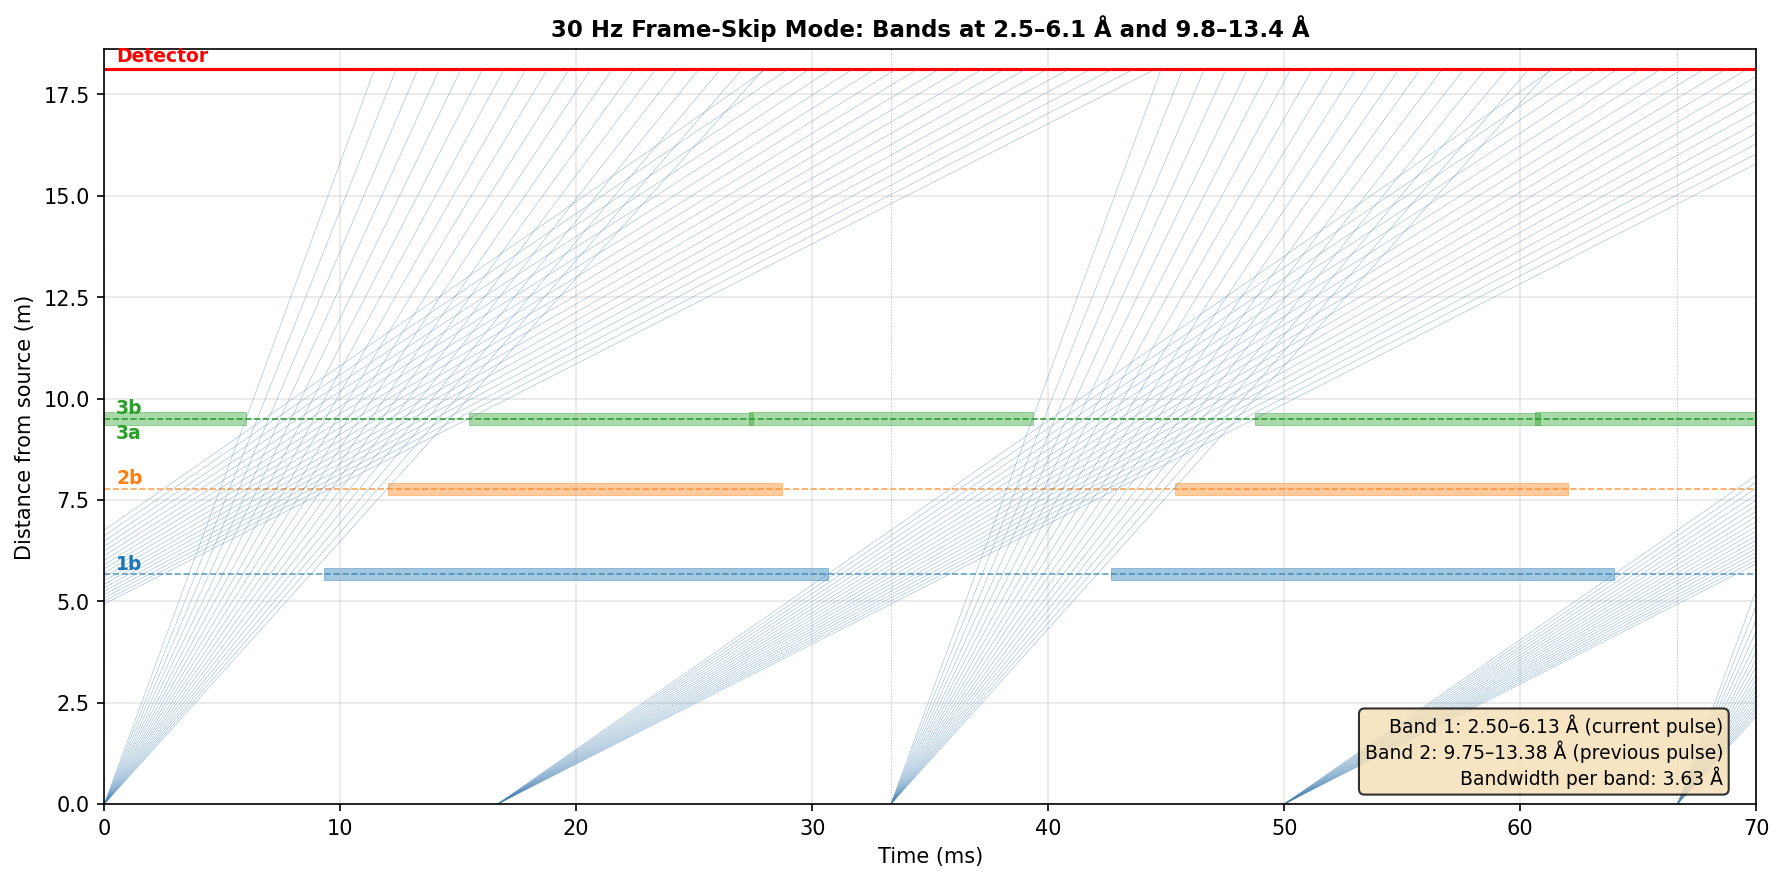
\includegraphics[width=5.5in]{figures/diagram_30hz.png}
    \longcaption{Distance--time diagram for 30\,Hz frame-skip mode.}{Two distinct wavelength bands are visible: Band~1 (2.5--6.1\,\AA{}) from the current pulse, and Band~2 (9.8--13.4\,\AA{}) from the previous pulse.}
    \label{fig:diagram_30hz}
\end{figure}

\subsection{Monochromatic Mode}

For applications requiring a narrow wavelength band centered on a specific wavelength, all six choppers can be used in monochromatic mode. In this mode, hexaSub calculates phases such that:
\begin{itemize}
    \item \textbf{``a'' choppers} (1a, 2a, 3a): Opening edge aligned to $\lambda_{\min}$
    \item \textbf{``b'' choppers} (1b, 2b, 3b): Closing edge aligned to $\lambda_{\max}$
\end{itemize}

Figure~\ref{fig:diagram_mono} shows a configuration for 10\,\AA{} with $\pm$10\% spread (9.5--10.5\,\AA{}).

\begin{figure}[ht]
    \centering
    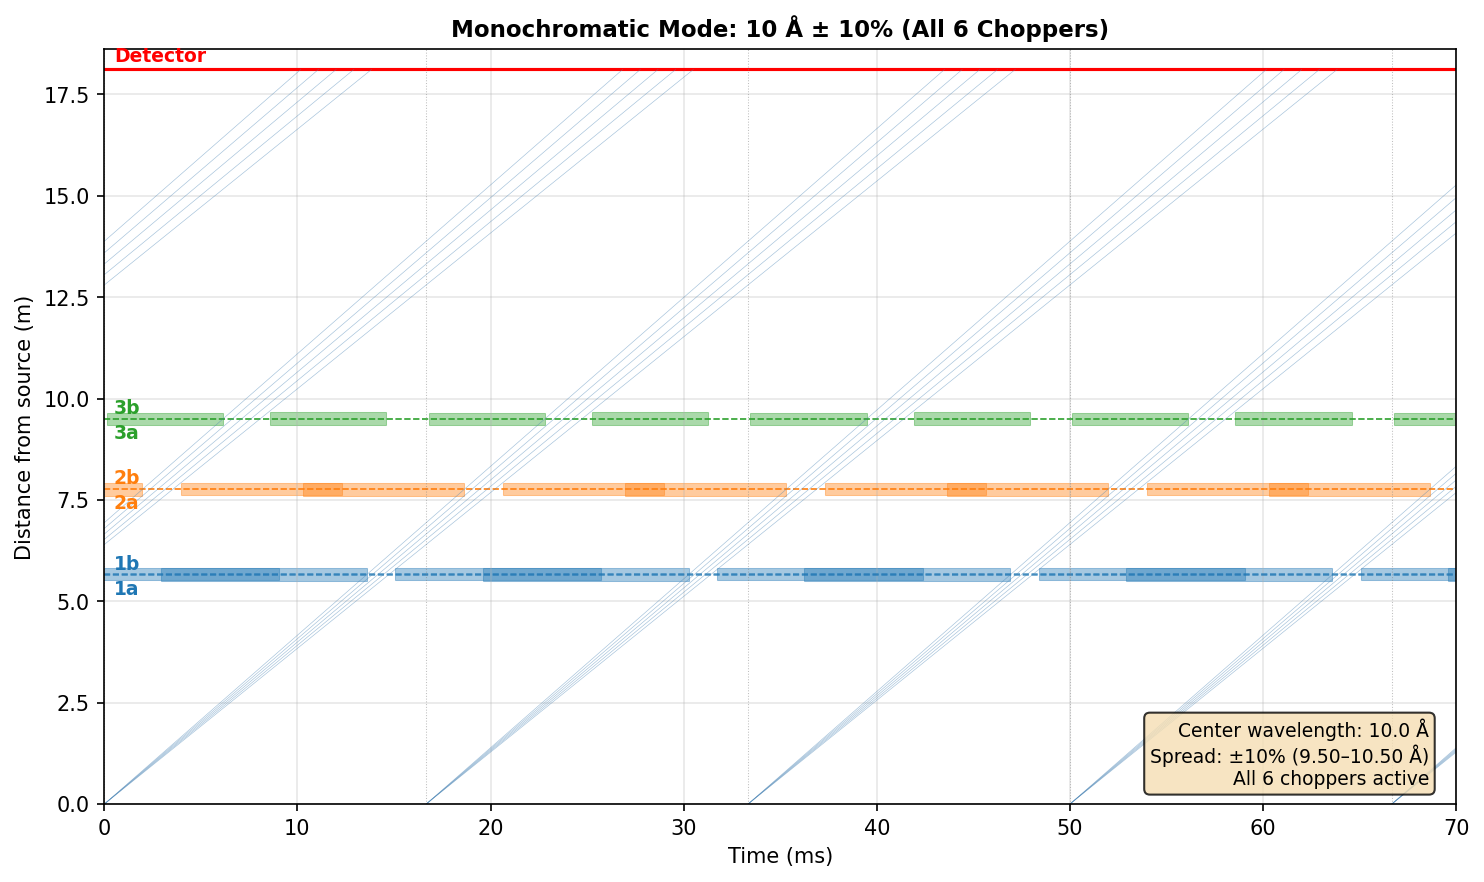
\includegraphics[width=5.5in]{figures/diagram_mono.png}
    \longcaption{Distance--time diagram for monochromatic mode: 10\,\AA{} $\pm$ 10\% (9.5--10.5\,\AA{}).}{All six choppers are active with phases calculated by hexaSub.}
    \label{fig:diagram_mono}
\end{figure}

%%%%%%%%%%%%%%%%%%%%%%%%%%%%%%%%%%%%%%%%%%%%%%%%%%%%%%%%%%%%%%%%%%%%%%%%%%%%%%%
\section{TOOL 1: INTERACTIVE EDGE FINDER}
%%%%%%%%%%%%%%%%%%%%%%%%%%%%%%%%%%%%%%%%%%%%%%%%%%%%%%%%%%%%%%%%%%%%%%%%%%%%%%%

\subsection{Purpose}

The \texttt{find\_edges\_ui.py} tool analyzes monitor spectra to:
\begin{itemize}
    \item Identify the TOF positions of chopper blade edges (rising/falling transitions)
    \item Fit edges using an error function (erf) model
    \item Calculate the phase offset between measured edges and expected chopper timing
\end{itemize}

\subsection{Starting the Tool}

\begin{lstlisting}[language=bash]
# Load spectrum from ASCII file (60 Hz mode)
python find_edges_ui.py 176475_monitor.dat

# Load spectrum in 30 Hz mode
python find_edges_ui.py --30hz 176550_monitor.dat

# Start without file (load via Phase Calculator)
python find_edges_ui.py
\end{lstlisting}

\subsection{User Interface Overview}

The interface consists of two windows (Figure~\ref{fig:find_edges_ui}):
\begin{enumerate}
    \item \textbf{Main Plot Window}: Displays the TOF spectrum with interactive edge marking
    \item \textbf{Phase Calculator Window}: Computes OGC and phase offsets from edge positions
\end{enumerate}

\begin{figure}[ht]
    \centering
    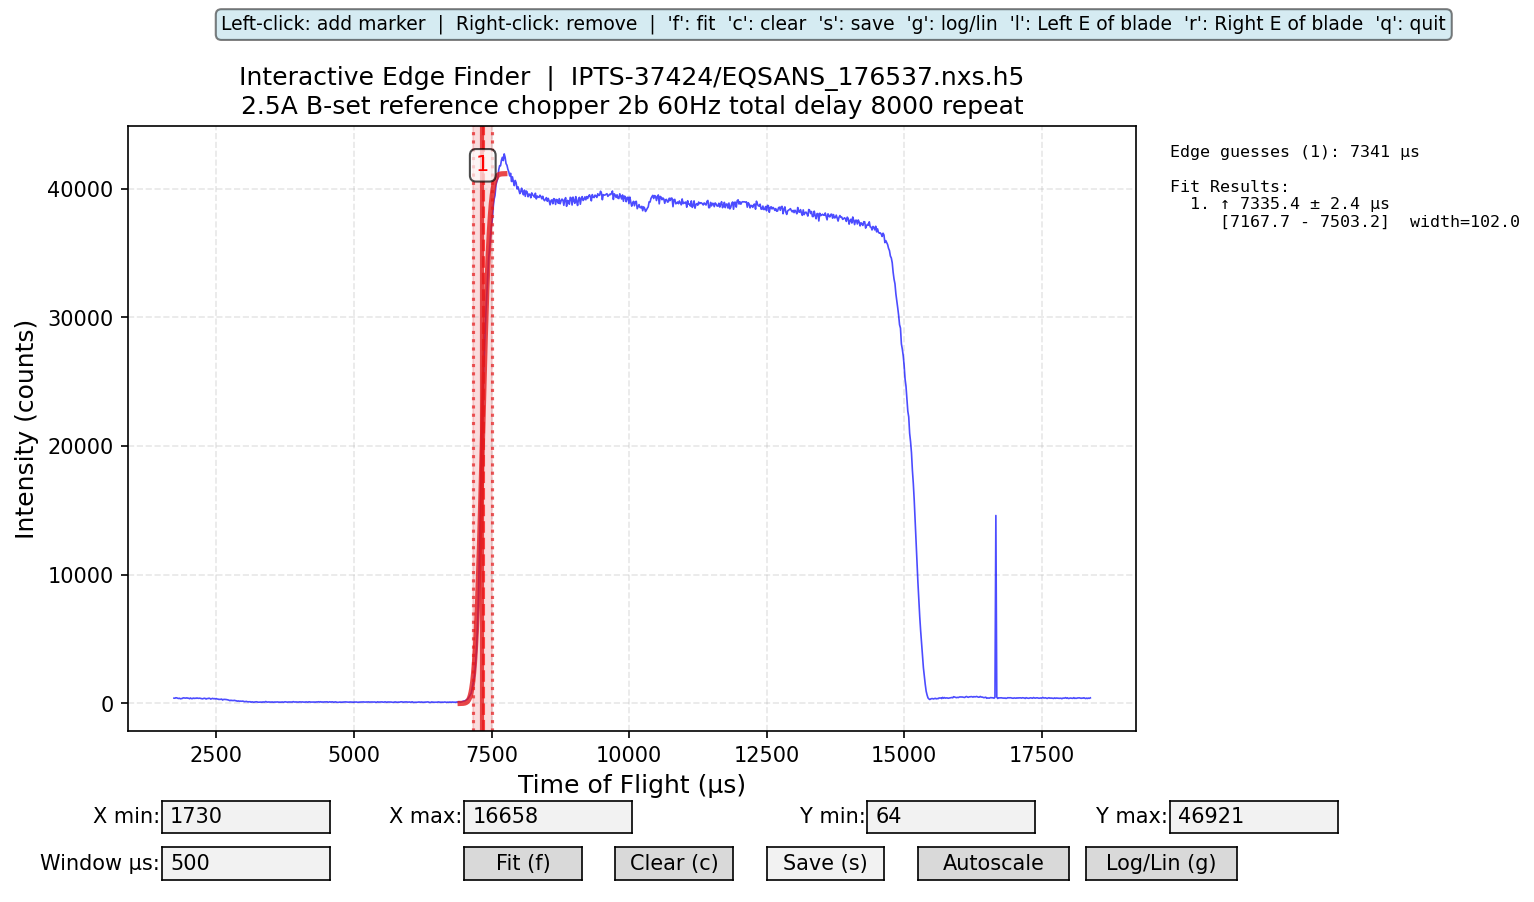
\includegraphics[width=5.5in]{figures/find_edges_60hz_example.png}
    \longcaption{Interactive Edge Finder showing a 60\,Hz monitor spectrum.}{The fit result panel shows the edge position (7335.4 $\pm$ 2.4\,$\mu$s), fit range, and transition width.}
    \label{fig:find_edges_ui}
\end{figure}

\subsection{Keyboard Shortcuts and Controls}

\begin{table}[ht]
\centering

\caption{Interactive Controls}
\label{tab:shortcuts}
\begin{tabular}{ll}
\toprule
Action & Control \\
\midrule
Add edge marker & Left-click on plot \\
Remove nearest marker & Right-click on plot \\
Fit all marked edges & Press \texttt{f} or click ``Fit'' \\
Clear all markers & Press \texttt{c} or click ``Clear'' \\
Save results (data + image) & Press \texttt{s} or click ``Save'' \\
Toggle log/linear Y-scale & Press \texttt{g} or click ``Log/Lin'' \\
Set left blade edge to cursor & Press \texttt{l} \\
Set right blade edge to cursor & Press \texttt{r} \\
Quit & Press \texttt{q} \\
\bottomrule
\end{tabular}

\end{table}

\subsection{Step-by-Step Workflow: Extracting Phase Offset}

\subsubsection{Step 1: Load the Monitor Spectrum}

\textbf{Option A --- From ASCII file}:
\begin{lstlisting}[language=bash]
python find_edges_ui.py edge_refinement/176505_monitor.dat
\end{lstlisting}

\textbf{Option B --- From NeXus via Phase Calculator}:
\begin{enumerate}
    \item Start the tool without a file: \texttt{python find\_edges\_ui.py}
    \item In the Phase Calculator window, enter the IPTS number and Run number
    \item Click ``Load'' to fetch the spectrum from the NeXus file
\end{enumerate}

\subsubsection{Step 2: Mark Edge Positions}

\begin{enumerate}
    \item Identify the rising and/or falling edges in the spectrum (transitions where intensity changes sharply)
    \item Left-click at each edge location to place a numbered marker
    \item Use right-click to remove incorrectly placed markers
\end{enumerate}

\subsubsection{Step 3: Fit the Edges}

Press \texttt{f} (or click ``Fit'') to fit all marked edges. The tool:
\begin{enumerate}
    \item Automatically detects whether each edge is rising or falling
    \item Fits an error function (erf) model to determine the precise edge position
    \item Displays the fit results: position $\pm$ uncertainty, width, and boundary region
\end{enumerate}

The erf model used for fitting is:
\begin{equation}
    I(t) = \frac{I_R - I_L}{2} \left[ 1 + \text{erf}\left(\frac{t - t_0}{\sqrt{2}\sigma}\right) \right] + I_L
\end{equation}
where $t_0$ is the edge position, $\sigma$ is the transition width, and $I_L$, $I_R$ are the left/right intensity levels.

\subsubsection{Step 4: Capture Edge Values for Phase Calculation}

\begin{enumerate}
    \item In the Phase Calculator, select the chopper being calibrated (e.g., 1b, 2a, etc.)
    \item Position the mouse cursor at the fitted edge position
    \item Press \texttt{l} to set as ``Left E of blade'' or \texttt{r} for ``Right E of blade''
    \item Alternatively, type the TOF value directly into the input field
\end{enumerate}

\subsubsection{Step 5: Read the Phase Offset}

The Phase Calculator computes and displays:
\begin{itemize}
    \item \textbf{OGC}: The Opening Gap Center time calculated from the edge position
    \item \textbf{Phase offset}: The difference between the current offset setting and the calculated OGC
\end{itemize}

The OGC is calculated as:
\begin{equation}
    \text{OGC} = \frac{L \cdot t_{\text{edge}}}{k} \pm \frac{\theta}{360°} \cdot \frac{T_{\text{period}}}{2}
\end{equation}
where the sign depends on whether it's the left (opening, $+$) or right (closing, $-$) edge.

\subsubsection{Step 6: Save Results}

Press \texttt{s} to save:
\begin{itemize}
    \item ASCII file with edge fit results (position, uncertainty, width, amplitude)
    \item PNG image of the spectrum with fitted edges
\end{itemize}

\subsection{Example: 30\,Hz Frame-Skip Mode}

Figure~\ref{fig:find_edges_30hz} shows edge detection in 30\,Hz mode, where the frame period extends to 33,333\,$\mu$s.

\begin{figure}[ht]
    \centering
    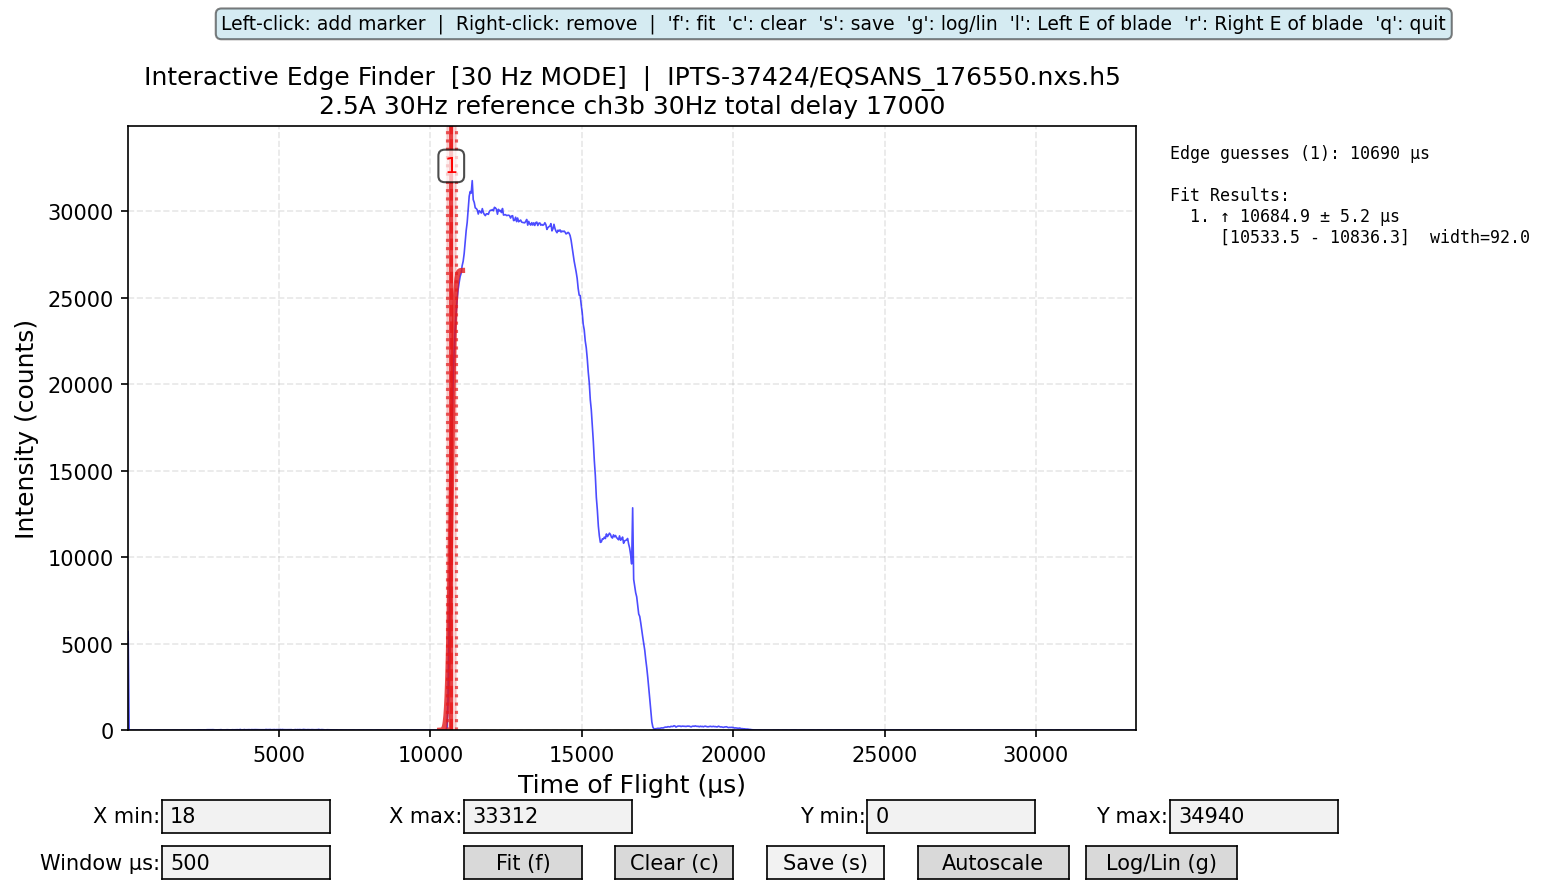
\includegraphics[width=5.5in]{figures/find_edges_30hz_example.png}
    \longcaption{Edge detection in 30\,Hz frame-skip mode.}{The extended TOF range (0--33,333\,$\mu$s) captures the full chopper period.}
    \label{fig:find_edges_30hz}
\end{figure}

%%%%%%%%%%%%%%%%%%%%%%%%%%%%%%%%%%%%%%%%%%%%%%%%%%%%%%%%%%%%%%%%%%%%%%%%%%%%%%%
\section{TOOL 2: MULTI-CHOPPER SIMULATOR}
%%%%%%%%%%%%%%%%%%%%%%%%%%%%%%%%%%%%%%%%%%%%%%%%%%%%%%%%%%%%%%%%%%%%%%%%%%%%%%%

\subsection{Purpose}

The \texttt{eqsans\_chopper\_sim.py} tool provides:
\begin{itemize}
    \item Visual simulation of neutron trajectories through multiple choppers
    \item Prediction of wavelength bands for given phase settings
    \item Verification that hexaSub-calculated phases produce expected results
    \item Distance--time diagrams showing chopper open/closed states
\end{itemize}

\subsection{Starting the Tool}

\begin{lstlisting}[language=bash]
python eqsans_chopper_sim.py
\end{lstlisting}

\subsection{User Interface Overview}

The simulator GUI consists of:
\begin{itemize}
    \item \textbf{Control Panel (left)}: Frequency selection, chopper enable/disable, OGC and mechanical offset inputs, hexaSub checkbox
    \item \textbf{Distance--Time Diagram (top right)}: Shows chopper positions, open/closed windows, and neutron trajectories
    \item \textbf{Detector TOF Spectrum (bottom right)}: Histogram of neutrons arriving at the detector
\end{itemize}

\subsection{Control Panel Elements}

\begin{table}[ht]
\centering

\caption{Simulator Controls}
\label{tab:sim_controls}
\begin{tabular}{lp{9cm}}
\toprule
Control & Description \\
\midrule
Detector distance & Physical distance from sample to detector (meters) \\
Frequency (60/30 Hz) & Chopper rotation frequency; affects period and frame-skip behavior \\
Chopper checkboxes & Enable/disable individual choppers in the simulation \\
OGC ($\mu$s) & Opening Gap Center phase for each chopper \\
Mech offset ($\mu$s) & Mechanical offset added to OGC (calibration correction) \\
hexaSub phases & When checked, auto-populates mech offsets for hexaSub compatibility \\
Calculate & Run the simulation with current settings \\
Log scale & Toggle logarithmic Y-axis on TOF spectrum \\
\bottomrule
\end{tabular}

\end{table}

\subsection{Understanding the hexaSub Checkbox}

The \ac{eqsans} chopper control system uses \texttt{hexaSub.c} to calculate OGC phases for a requested wavelength. These phases include hardware calibration offsets ($\sim$29,000--30,000\,$\mu$s) that account for encoder alignment, cable delays, and other instrument-specific factors.

When the \textbf{hexaSub phases} checkbox is enabled:
\begin{enumerate}
    \item The simulator automatically sets mechanical offsets to compensate for hexaSub calibration
    \item For 30\,Hz mode, additional frame-skip alignment corrections are applied
    \item You can directly paste hexaSub OGC values into the OGC fields
\end{enumerate}

Table~\ref{tab:hexasub_offsets} shows the mechanical offsets applied for 30\,Hz mode.

\begin{table}[ht]
\centering

\caption{Mechanical Offsets with hexaSub Checkbox (30\,Hz Mode)}
\label{tab:hexasub_offsets}
\begin{tabular}{lccc}
\toprule
Chopper & Calibration Offset ($\mu$s) & Frame-skip Align ($\mu$s) & Net Mech Offset ($\mu$s) \\
\midrule
1b & $-29908.92$ & $0$ & $-29908.92$ \\
2b & $-29610.80$ & $0$ & $-29610.80$ \\
3a & $-29452.12$ & $+33333.33$ & $+3881.21$ \\
3b & $-29131.20$ & $+33333.33$ & $+4202.13$ \\
\bottomrule
\end{tabular}

\end{table}

\subsection{Step-by-Step Workflow: Verifying hexaSub Phases}

\subsubsection{Step 1: Configure the Frequency}

Select \textbf{30 Hz} or \textbf{60 Hz} to match the chopper operating mode.

\subsubsection{Step 2: Enable the Appropriate Choppers}

For 30\,Hz frame-skip mode, enable choppers \textbf{1b, 2b, 3a, 3b} (the ``b-set'' plus 3a/3b).

\subsubsection{Step 3: Enable hexaSub Phases}

Check the \textbf{hexaSub phases} checkbox. This automatically sets the mechanical offsets.

\subsubsection{Step 4: Enter hexaSub OGC Values}

Enter the OGC values calculated by hexaSub for your wavelength setting. For example, for 2.5\,\AA{} at 30\,Hz with SDD=4\,m:

\begin{table}[ht]
\centering
\begin{tabular}{lc}
\toprule
Chopper & hexaSub OGC ($\mu$s) \\
\midrule
1b & 33233.61 \\
2b & 33318.81 \\
3a & 921.45 \\
3b & 12454.81 \\
\bottomrule
\end{tabular}
\end{table}

\subsubsection{Step 5: Run the Simulation}

Click \textbf{Calculate}. The simulator will display:
\begin{itemize}
    \item Distance--time diagram with chopper windows and neutron trajectories
    \item Detector TOF spectrum showing the wavelength bands that pass
\end{itemize}

\subsubsection{Step 6: Verify the Results}

For the 2.5\,\AA{} @ 30\,Hz example, you should see two wavelength bands:
\begin{itemize}
    \item \textbf{Band 1}: $\sim$2.5--6.1\,\AA{} (from current source pulse)
    \item \textbf{Band 2}: $\sim$9.8--13.4\,\AA{} (from previous source pulse)
\end{itemize}

The status bar reports the number of pulse groups that passed and the peak TOF.

\subsection{Understanding the Distance--Time Diagram}

The diagram shows:
\begin{itemize}
    \item \textbf{Horizontal axis}: Time (ms) from source pulse
    \item \textbf{Vertical axis}: Distance from source (m)
    \item \textbf{Shaded rectangles}: Chopper closed periods (color-coded by chopper)
    \item \textbf{Horizontal dashed lines}: Chopper positions with labels showing name, distance, and effective OGC
    \item \textbf{Blue trajectory lines}: Sampled neutron paths that successfully pass all choppers
    \item \textbf{Top line}: Detector position
\end{itemize}

Neutrons that intersect a shaded (closed) region are blocked. Only trajectories passing through all open windows reach the detector.

\subsection{Relationship to hexaSub.c}

The \texttt{hexaSub.c} code in the EPICS IOC calculates chopper phases using the \texttt{calc6Phases()} function. This section provides detailed explanations of phase calculation for all three operating modes.

\subsubsection{Common Elements}

All modes share these fundamental calculations:

\begin{itemize}
    \item \textbf{TOF calculation}: Time-of-flight from source to chopper position using $\text{TOF} = d / (3956 \times 10^3) \times \lambda$ where $d$ is in mm and $\lambda$ in \AA{}
    
    \item \textbf{Centering adjustment}: After aligning an edge to a wavelength, the phase is adjusted by $\pm \theta_{\text{opening}} \times t_{\text{half-angle}}$ to center the OGC (Opening Gap Center) on the opening window
    
    \item \textbf{Calibration offset}: Hardware-specific offset ($\sim$15,000\,$\mu$s at 60\,Hz, $\sim$30,000\,$\mu$s at 30\,Hz) added to account for encoder alignment, cable delays, etc.
    
    \item \textbf{Period wrapping}: Final phase wrapped to one period via \texttt{fmod(phase, frame\_width)}
\end{itemize}

The general formula for each chopper is:
\begin{equation}
\text{OGC} = \texttt{fmod}\Big( 10^6 \times \big( \text{TOF}_\lambda \pm \theta_{\text{opening}} \times t_{\text{half-angle}} \big) + \text{offset}_{\text{cal}} \,,\; T_{\text{frame}} \Big)
\end{equation}

\subsubsection{60\,Hz Mode (Standard Operation)}

In 60\,Hz mode, hexaSub uses choppers indexed 1--6 in the code. The array index mapping is:

\begin{center}
\texttt{index: 1=1b, 2=2b, 3=3a, 4=3b, 5=1a, 6=2a}
\end{center}

The phase offsets are:

\begin{verbatim}
phase_offset[] = {0, 14954.46, 14805.4, 14726.06, 14565.69, 15072.89, 14834.04}
                    (1b)       (2b)      (3a)      (3b)      (1a)      (2a)
\end{verbatim}

\textbf{Wavelength-dependent alignment (critical)}:

The 60\,Hz mode has \emph{different} alignment logic depending on whether $\lambda_1 > 13$\,\AA{}:

\begin{table}[ht]
\centering

\caption{60\,Hz Mode Edge Alignment}
\label{tab:60hz_alignment}
\begin{tabular}{lcccc}
\toprule
Condition & 1a/1b Edge & Aligned to & 2a/2b Edge & Aligned to \\
\midrule
$\lambda_1 > 13$\,\AA{} & Opening & $\lambda_1$ & Closing & $\lambda_2$ \\
$\lambda_1 \leq 13$\,\AA{} & Closing & $\lambda_2$ & Opening & $\lambda_1$ \\
\bottomrule
\end{tabular}

\end{table}

This swap prevents neutron leakage at different wavelength ranges. The choppers 3a and 3b do \emph{not} swap:
\begin{itemize}
    \item \textbf{3a}: Closing edge always aligned to $\lambda_2$ (band end)
    \item \textbf{3b}: Opening edge always aligned to $\lambda_1$ (band start)
\end{itemize}

\textbf{Phase calculation (60\,Hz)}:

For $\lambda_1 \leq 13$\,\AA{} (most common):
\begin{align}
\text{phase}_{1\text{a/b}} &= \text{TOF}(\lambda_2) - \theta_{\text{open}} \times t_{\text{half}} + \text{offset} \quad \text{(closing edge)} \\
\text{phase}_{2\text{a/b}} &= \text{TOF}(\lambda_1) + \theta_{\text{open}} \times t_{\text{half}} + \text{offset} \quad \text{(opening edge)} \\
\text{phase}_{3\text{a}} &= \text{TOF}(\lambda_2) - \theta_{\text{open}} \times t_{\text{half}} + \text{offset} \quad \text{(closing edge)} \\
\text{phase}_{3\text{b}} &= \text{TOF}(\lambda_1) + \theta_{\text{open}} \times t_{\text{half}} + \text{offset} \quad \text{(opening edge)}
\end{align}

\subsubsection{30\,Hz Frame-Skip Mode}

In 30\,Hz mode, choppers rotate at half speed, allowing two source pulses to contribute per chopper period. This creates \emph{two} wavelength bands. Only choppers 1b, 2b, 3a, 3b are used (indices 1, 2, 3, 4).

\textbf{Phase offsets (30\,Hz)}:

The 30\,Hz phase offsets are exactly \emph{double} the 60\,Hz values:

\begin{verbatim}
phase_offset[] = {0, 29908.92, 29610.80, 29452.12, 29131.38, 30145.78, 29668.08}
                    (1b)       (2b)       (3a)      (3b)      (1a)      (2a)
\end{verbatim}

This is $2 \times$ the 60\,Hz offsets because the chopper period doubles from 16,666.67\,$\mu$s to 33,333.33\,$\mu$s.

\textbf{Wavelength bands}:

hexaSub computes four wavelengths for frame-skip mode:
\begin{itemize}
    \item $\lambda_1$: Band 1 start (user-requested wavelength)
    \item $\lambda_2 = \lambda_1 + \Delta\lambda_{60\text{Hz}}$: Band 1 end
    \item $\lambda_3 = \lambda_2 + \Delta\lambda_{60\text{Hz}}$: Band 2 start  
    \item $\lambda_4 = \lambda_3 + \Delta\lambda_{60\text{Hz}}$: Band 2 end
\end{itemize}

\textbf{Pulse alignment (critical)}:

Different choppers align to \emph{different} source pulses:

\begin{table}[ht]
\centering

\caption{30\,Hz Mode Chopper Alignment}
\label{tab:30hz_alignment}
\begin{tabular}{lccc}
\toprule
Chopper & Edge Type & Wavelength & Source Pulse \\
\midrule
1b (index 1) & Opening & $\lambda_3$ & Previous ($-1/60$\,s) \\
2b (index 2) & Closing & $\lambda_2$ & Current \\
3a (index 3) & Closing & $\lambda_4$ & Previous ($-1/60$\,s) \\
3b (index 4) & Opening & $\lambda_1$ & Current \\
\bottomrule
\end{tabular}

\end{table}

The ``previous pulse'' alignment means the TOF calculation \emph{always} includes subtraction of $1/60$\,s (one source period) for choppers 1b and 3a:

\begin{verbatim}
// For choppers 1b (index 1) and 1a (index 5):
phase = tof - 1.0/60.0;  // Always subtract, regardless of tof value

// For chopper 3a (index 3):
phase = tof - 1.0/60.0;  // Always subtract
\end{verbatim}

This creates the frame-skip behavior where Band 2 neutrons (longer wavelengths) from the \emph{previous} source pulse arrive at the detector in the same time window as Band 1 neutrons from the \emph{current} pulse.

\textbf{Simulator frame-skip corrections}:

When using hexaSub phases in the simulator (checkbox enabled), frame-skip alignment corrections are applied only for choppers 3a and 3b:
\begin{itemize}
    \item 3a: $+33333.33$\,$\mu$s (full 30\,Hz period)
    \item 3b: $+33333.33$\,$\mu$s (full 30\,Hz period)
\end{itemize}

These corrections compensate for the period-wrapping in hexaSub's \texttt{fmod()} operation. Choppers 1b and 2b require no additional alignment correction because hexaSub always subtracts $1/60$\,s for 1b, resulting in phase values that already account for pulse alignment.

\subsubsection{Monochromatic Mode}

Monochromatic mode uses all six choppers to produce a narrow wavelength band (e.g., 10\,\AA{} $\pm$10\%). This mode operates at 60\,Hz and uses the 60\,Hz phase offsets.

\textbf{Phase offsets (same as 60\,Hz)}:
\begin{verbatim}
phase_offset[] = {0, 14954.46, 14805.4, 14726.06, 14565.69, 15072.89, 14834.04}
                    (1b)       (2b)      (3a)      (3b)      (1a)      (2a)
\end{verbatim}

\textbf{Simple alignment rule}:

Unlike the 60\,Hz standard mode, monochromatic mode has \emph{no} wavelength-dependent switching:
\begin{itemize}
    \item \textbf{All ``a'' choppers} (1a, 2a, 3a): Opening edge aligned to $\lambda_{\min}$
    \item \textbf{All ``b'' choppers} (1b, 2b, 3b): Closing edge aligned to $\lambda_{\max}$
\end{itemize}

\begin{table}[ht]
\centering

\caption{Monochromatic Mode Edge Alignment}
\label{tab:mono_alignment}
\begin{tabular}{lcc}
\toprule
Chopper & Edge Type & Aligned to \\
\midrule
1b (index 1) & Closing & $\lambda_{\max}$ \\
2b (index 2) & Closing & $\lambda_{\max}$ \\
3a (index 3) & Opening & $\lambda_{\min}$ \\
3b (index 4) & Closing & $\lambda_{\max}$ \\
1a (index 5) & Opening & $\lambda_{\min}$ \\
2a (index 6) & Opening & $\lambda_{\min}$ \\
\bottomrule
\end{tabular}

\end{table}

\textbf{Phase calculation (monochromatic)}:

\begin{align}
\text{phase}_{n\text{a}} &= \text{TOF}(\lambda_{\min}) + \theta_{\text{open}} \times t_{\text{half}} + \text{offset} \quad \text{(opening edge)} \\
\text{phase}_{n\text{b}} &= \text{TOF}(\lambda_{\max}) - \theta_{\text{open}} \times t_{\text{half}} + \text{offset} \quad \text{(closing edge)}
\end{align}

\subsubsection{Summary: Mode Comparison}

\begin{table}[ht]
\centering

\caption{Comparison of hexaSub Operating Modes}
\label{tab:mode_comparison}
\begin{tabular}{lccc}
\toprule
Feature & 60\,Hz Standard & 30\,Hz Frame-Skip & Monochromatic \\
\midrule
Chopper speed & 60\,Hz & 30\,Hz & 60\,Hz \\
Choppers used & 4 (1a/b, 2a/b or 3a/b) & 4 (1b, 2b, 3a, 3b) & 6 (all) \\
Wavelength bands & 1 & 2 & 1 (narrow) \\
Phase offsets & $\sim$15,000\,$\mu$s & $\sim$30,000\,$\mu$s & $\sim$15,000\,$\mu$s \\
$\lambda > 13$\,\AA{} switch & Yes & No & No \\
Pulse alignment & Single pulse & Split (prev/curr) & Single pulse \\
\bottomrule
\end{tabular}

\end{table}

%%%%%%%%%%%%%%%%%%%%%%%%%%%%%%%%%%%%%%%%%%%%%%%%%%%%%%%%%%%%%%%%%%%%%%%%%%%%%%%
\section{PRACTICAL EXAMPLES}
%%%%%%%%%%%%%%%%%%%%%%%%%%%%%%%%%%%%%%%%%%%%%%%%%%%%%%%%%%%%%%%%%%%%%%%%%%%%%%%

\subsection{Example 1: Single Chopper Calibration (60\,Hz)}

\textbf{Goal}: Determine the phase offset for chopper 1b from a calibration run.

\begin{enumerate}
    \item Acquire a monitor spectrum with only chopper 1b active
    \item Load the spectrum: \texttt{python find\_edges\_ui.py 176479\_1b\_pd1000\_monitor.dat}
    \item Identify and mark the rising and falling edges
    \item Press \texttt{f} to fit both edges
    \item In Phase Calculator, select ``1b'' and capture each edge using \texttt{l} and \texttt{r}
    \item Record the phase offset values for left and right edges
    \item The average offset indicates the calibration correction needed
\end{enumerate}

\subsection{Example 2: Verifying 30\,Hz Frame-Skip Configuration}

\textbf{Goal}: Confirm that hexaSub phases for 2.5\,\AA{} @ 30\,Hz produce the expected bands.

\begin{enumerate}
    \item Start the simulator: \texttt{python eqsans\_chopper\_sim.py}
    \item Select \textbf{30 Hz} frequency
    \item Enable choppers 1b, 2b, 3a, 3b (disable 1a, 2a)
    \item Check \textbf{hexaSub phases}
    \item Enter OGC values: 1b=33233.61, 2b=33318.81, 3a=921.45, 3b=12454.81
    \item Click \textbf{Calculate}
    \item Verify two bands appear: $\sim$2.5--6.1\,\AA{} and $\sim$9.8--13.4\,\AA{}
\end{enumerate}

\subsection{Example 3: Diagnosing Phase Mismatch}

\textbf{Symptom}: Measured wavelength band doesn't match expected range.

\textbf{Diagnostic workflow}:
\begin{enumerate}
    \item Use \texttt{find\_edges\_ui.py} to measure actual edge positions from monitor data
    \item Compare measured edges to hexaSub-predicted values
    \item In the simulator, enter the \emph{measured} OGC values (with hexaSub checkbox \emph{off})
    \item Observe which wavelengths pass --- this shows the actual instrument state
    \item The difference between expected and measured OGC indicates the calibration drift
\end{enumerate}

%%%%%%%%%%%%%%%%%%%%%%%%%%%%%%%%%%%%%%%%%%%%%%%%%%%%%%%%%%%%%%%%%%%%%%%%%%%%%%%
\section{TROUBLESHOOTING}
%%%%%%%%%%%%%%%%%%%%%%%%%%%%%%%%%%%%%%%%%%%%%%%%%%%%%%%%%%%%%%%%%%%%%%%%%%%%%%%

\subsection{No Wavelengths Pass in Simulator}

\begin{itemize}
    \item Check that choppers are enabled (checkboxes)
    \item Verify OGC values are reasonable (typically 0--33,333\,$\mu$s for 30\,Hz)
    \item If using hexaSub phases, ensure the checkbox is checked
    \item Try with only one or two choppers to isolate timing issues
\end{itemize}

\subsection{Edge Fit Fails}

\begin{itemize}
    \item Increase the ``Window'' parameter to include more data around the edge
    \item Ensure the marker is placed near the actual transition, not on flat regions
    \item Check that the spectrum has sufficient statistics (low-count data may not fit well)
\end{itemize}

\subsection{Phase Calculator Shows Unexpected Values}

\begin{itemize}
    \item Verify the correct chopper is selected
    \item Check that 30\,Hz mode is enabled if using 30\,Hz data (title shows ``[30 Hz MODE]'')
    \item Confirm the ``Current offset'' field contains the expected value for comparison
\end{itemize}

%%%%%%%%%%%%%%%%%%%%%%%%%%%%%%%%%%%%%%%%%%%%%%%%%%%%%%%%%%%%%%%%%%%%%%%%%%%%%%%
\section{FILE FORMATS}
%%%%%%%%%%%%%%%%%%%%%%%%%%%%%%%%%%%%%%%%%%%%%%%%%%%%%%%%%%%%%%%%%%%%%%%%%%%%%%%

\subsection{Monitor Spectrum (.dat)}

ASCII format with two columns:
\begin{lstlisting}
# Optional title line starting with #
TOF_us    Intensity
1000.0    523
1010.0    547
...
\end{lstlisting}

\subsection{Edge Fit Results (.dat)}

Output from \texttt{find\_edges\_ui.py} save function:
\begin{lstlisting}
# Edge Detection Results (Interactive UI)
# Columns: edge_num edge_type position position_err start end width amplitude
1 rising 7335.4499 2.4172 7167.7388 7503.1609 101.9611 41168.3902
\end{lstlisting}

%%%%%%%%%%%%%%%%%%%%%%%%%%%%%%%%%%%%%%%%%%%%%%%%%%%%%%%%%%%%%%%%%%%%%%%%%%%%%%%
\section{REFERENCES}
%%%%%%%%%%%%%%%%%%%%%%%%%%%%%%%%%%%%%%%%%%%%%%%%%%%%%%%%%%%%%%%%%%%%%%%%%%%%%%%

\begin{itemize}
    \item \ac{eqsans} Instrument: \href{https://neutrons.ornl.gov/eqsans}{https://neutrons.ornl.gov/eqsans}
    \item hexaSub.c source: \texttt{bl6chopper\_src/hexaSub.c}
    \item Tool source code: \texttt{/EQSANS/shared/script/choppers/}
\end{itemize}

%%%%%%%%%%%%%%%%%%%%%%%%%%%%%%%%%%%%%%%%%%%%%%%%%%%%%%%%%%%%%%%%%%%%%%%%%%%%%%%
% Back cover
\backmatter

%%%%%%%%%%%%%%%%%%%%%%%%%%%%%%%%%%%%%%%%%%%%%%%%%%%%%%%%%%%%%%%%%%%%%%%%%%%%%%%
\end{document}
